\newpage
\section[Grating and Spectra]{Grating and Spectra (光栅与光谱)}

\subsection{Diffraction by a Double Slit}

\subsubsection{interference vs Diffraction}
\begin{enumerate}
    \item Let $a\rightarrow 0$, then $\alpha \rightarrow 0$ and $\frac{\sin\alpha}{\alpha}\rightarrow 1$, the equation just describes the interference pattern. 
    \item Let $d\rightarrow 0$, then $\beta \rightarrow 0$ and $\cos^2\beta\rightarrow 1$, the equation just describes the diffraction pattern. 
\end{enumerate}

If the combining waves originate from a small number of elementary coherent sources (as in a double-slit experiment with $\alpha \ll \lambda$ ), we call the process interference. 

If the combining waves originate in a single wavefront (as in a single-slit experiment), we call the process diffraction.  

\subsection{Diffraction Gratings}
in doble-slit interference with $a\ll \lambda$
\begin{align*}
    I(\theta)=I_{max}\cos^2\left[ \frac{\pi d}{\lambda}\sin \theta \right]
\end{align*}
The bright fringes due to different wavelengths overlap too much to be distinguished. 

A useful tool in the study of light and of objects that emit and absorb light is the \highlight{diffraction grating}, which has a much greater number $N$ of slits, often called \highlight{rulings (裁定)}, perhaps as many as several thousand per millimeter.

\subsubsection{Mutiple Slits with Monochromatic Light}
With monochromatic light incident on $N=2 \sim 6$ long narrow slits with slit-separation $d$, the normalized intensity (irradiance) evolves with sharper and sharper peaks. The phase difference between adjacent slits is 
\begin{align*}
    \delta_N =\frac{2\pi}{\lambda}\sin\theta
\end{align*}

\begin{figure}[H]
    \centering
    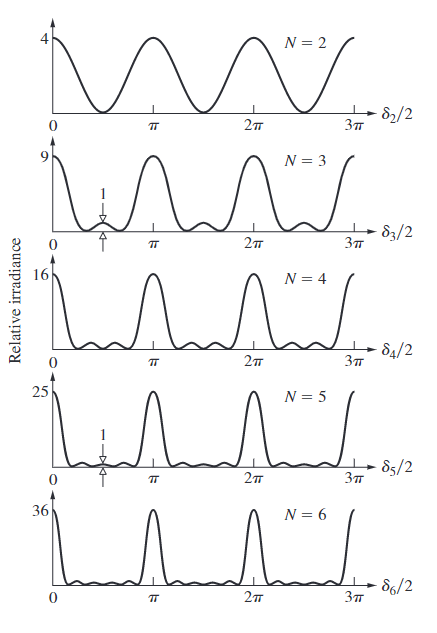
\includegraphics[width=0.109\textwidth]{Lec19/with monochromatic light incident on N = 2 to 6}
    \caption{with monochromatic light incident on N = 2 to 6}
\end{figure}


This case is for $N=4$
\begin{align*}
    \tilde{E}_{\theta}=E_0\left( e^{-3i\frac{\delta_4}{2}} + e^{-i\frac{\delta_4}{2}} + e^{i\frac{\delta_4}{2}} + e^{3i\frac{\delta_4}{2}}\right)
\end{align*}

\begin{figure}[H]
    \centering
    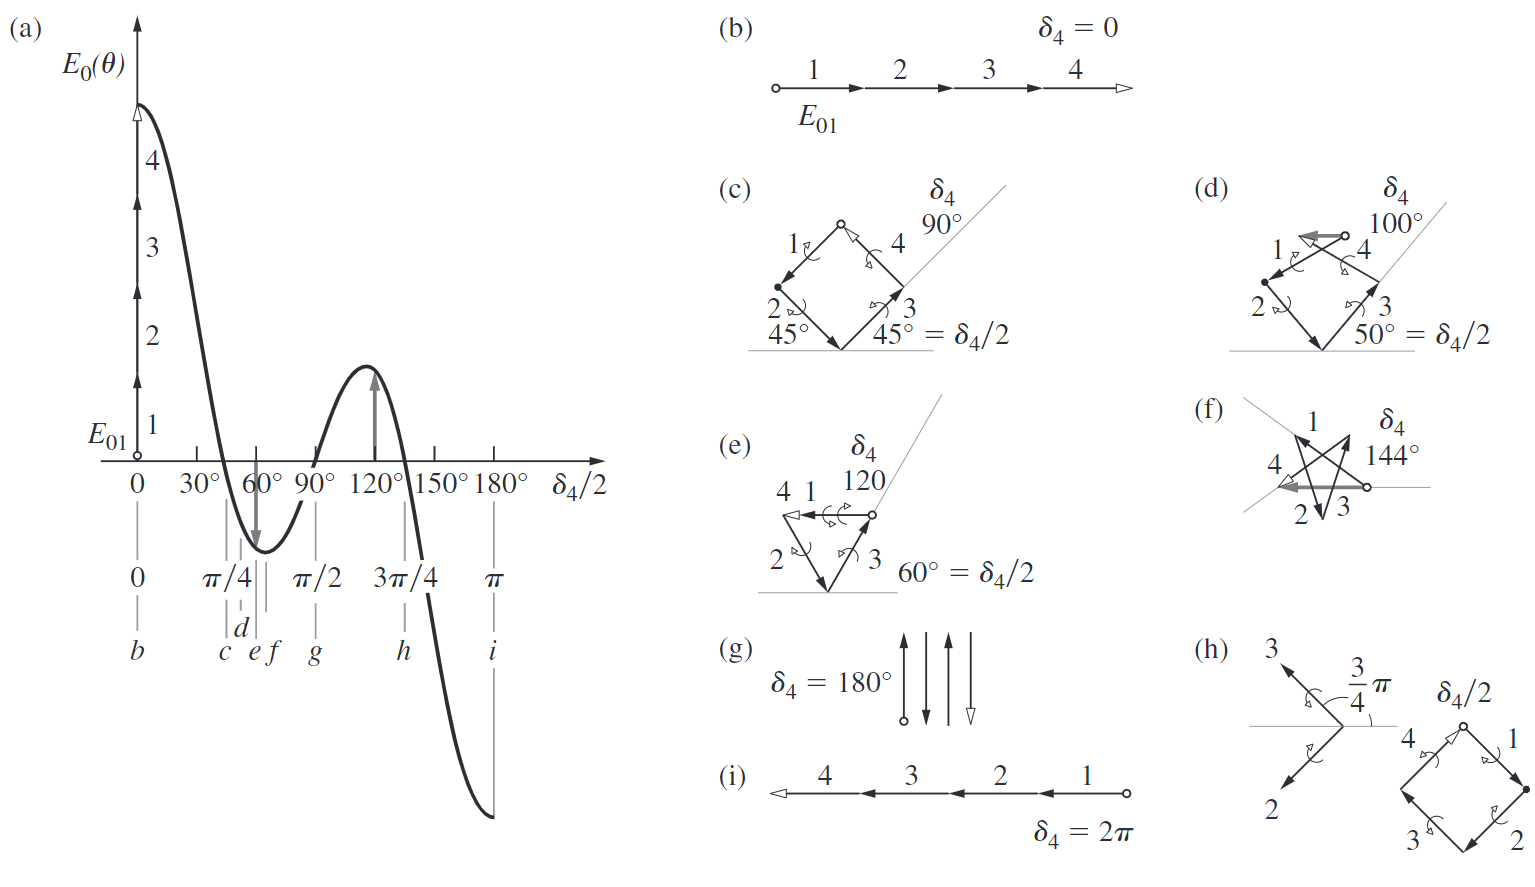
\includegraphics[width=0.48\textwidth]{Lec19/with monochromatic light incident on N = 4}
    \caption{with monochromatic light incident on N = 4}
\end{figure}

With monochromatic (red) light incident on a diffraction grating (with a large number $N$), we can see on a viewing screen very narrow (and so are called \highlight{lines}). These lines correspond to 
\begin{align*}
    &\delta_N=\frac{2\pi}{\lambda}\sin\theta=2\pi m\\
    \text{or } &d\sin\theta = m \lambda 
\end{align*}
They are separated by relatively wide dark regions. 

\subsubsection{Width of the Lines}
A grating's ability to resolve (separate) lines of different wavelengths depends on the linewidth. The \highlight{half-width} of the central line $\Delta \theta_{hw}$ is determined by the first minimum in intensity, at which the $N$ rays from the $N$ slits of the grating cancel one another. The first minimum occurs where the phase difference bewteen the adjacent slits is 
\begin{align*}
    \delta_N=&\frac{2\pi}{\lambda}\sin\Delta\theta_{hw}=\frac{2\pi}{N}\\
    \text{or } \Delta\theta_{hw}=&\frac{\lambda}{Nd}
\end{align*}

Note that for light of a given wavelength $\lambda$ and a given ruling separation $d$, the linewidths decrease with increasing $N$ and so reduce overlap. Therefore, light of several unknown wavelengths can be distinguished and identified by a grating. For example, the light emitted by a hydrogen lamp, which contains hydrogen gas, has four discrete wavelengths in the visble range
\begin{figure}[H]
    \centering
    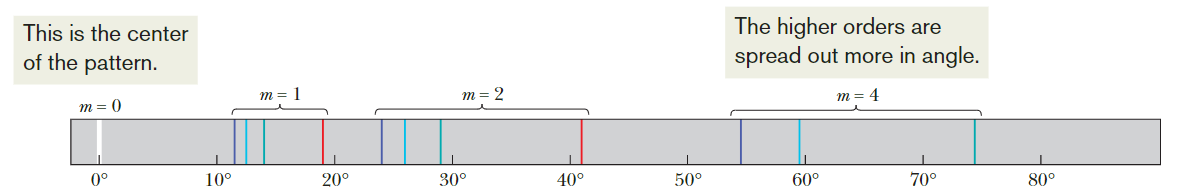
\includegraphics[width=0.309\textwidth]{Lec19/Hydrogen Spectra}
    \caption{Hydrogen Spectra}
\end{figure}

\subsubsection{Atomic Grating}
A crystalline solid, which consists of a regular array of atoms, resembles a diffraction grating with separation $d$ on the atomic scale $(\sim 10^{-10} m)$. Waves can be diffracted as if they were reflected by a family of parallel planes, with angles measured relative to the planes (not to a normal as in optics). 

\begin{figure}[H]
    \centering
    \begin{subfigure}{0.15\textwidth}
        \centering
        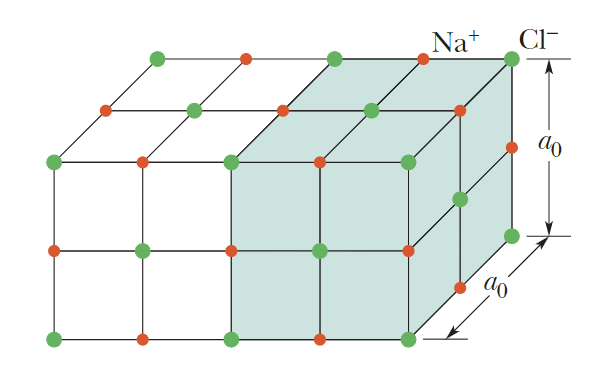
\includegraphics[width=\textwidth]{Lec19/Atomic Grating 1}

    \end{subfigure}
    \begin{subfigure}{0.15\textwidth}
        \centering
        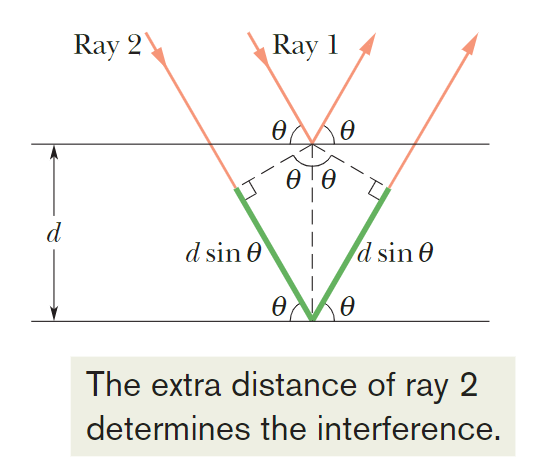
\includegraphics[width=\textwidth]{Lec19/Atomic Grating 2}

    \end{subfigure}
    \caption{Atomic Grating}
\end{figure}


% \begin{figure}[H]
%     \centering
%     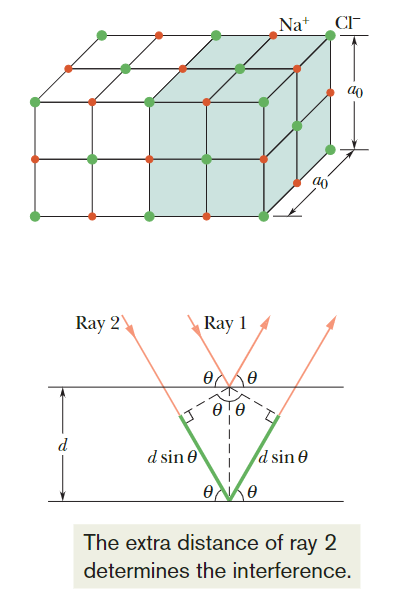
\includegraphics[width=0.209\textwidth]{Lec19/Atomic Grating}
%     \caption{Atomic Grating}
% \end{figure}

Suppose we would like to use the visble light $(\lambda \simeq 5.5 \times 10^{-7} m)$ to study the diffraction. The first-order mximum $(m=1)$ would occur at 
\begin{align*}
    \sin\theta=\frac{m\lambda}{2d}=2750 \gg 1
\end{align*}
This means that we wouldn't observe the first-order maxima. Therefore, we need waves with much shorter wavelength $(\lambda \approx d)$, that is, X rays. 

\subsection{X-Ray Diffraction}
X rays are electromagnetic radiation whose wavelengths are of the order of $10^{-10}m$. 

When an X-rays beam enters a crystal such as NaCl, X rays are scattered in all directions by the crystal structure. In some directions teh scattered waves unergos \highlight{destructive interference}, resulting in intensity minima; in other directions the interference is \highlight{constructive}, resulting in intensity maxima. 

\begin{figure}[H]
    \centering
    \begin{subfigure}{0.15\textwidth}
        \centering
        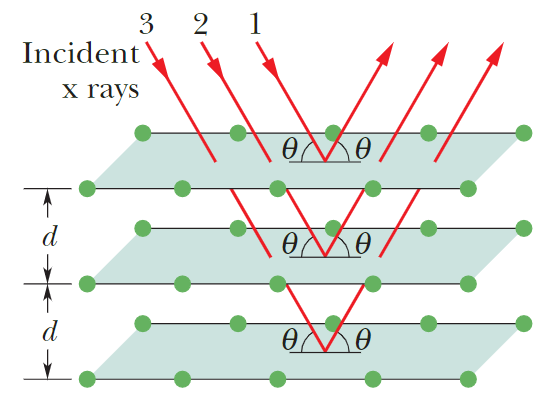
\includegraphics[width=\textwidth]{Lec19/X-Ray Diffraction 1}
    \end{subfigure}
    \begin{subfigure}{0.15\textwidth}
        \centering
        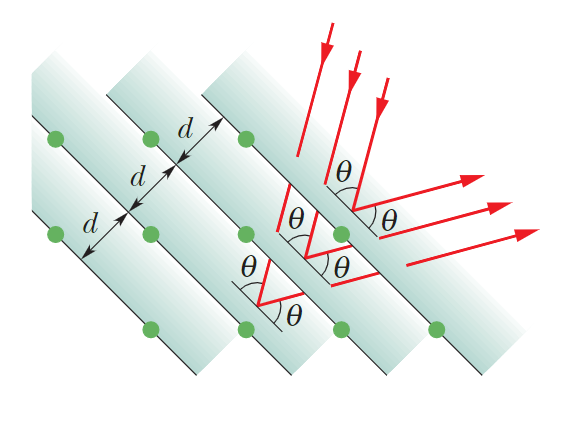
\includegraphics[width=\textwidth]{Lec19/X-Ray Diffraction 2}
    \end{subfigure}
    \caption{X-Ray Diffraction}
\end{figure}


% \begin{figure}[H]
%     \centering
%     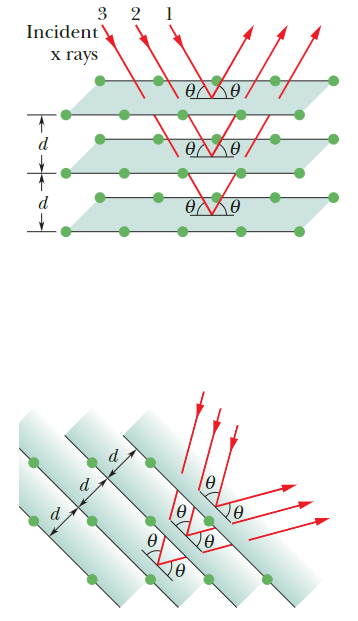
\includegraphics[width=0.159\textwidth]{Lec19/X-Ray Diffraction}
%     \caption{X-Ray Diffraction}
% \end{figure}

The maxima turn out to be in directions as if the X rays were reflected by a family of crystal planes that extend through the atoms within the crystal and that contain regular arrays of the atoms. \highlight{Bragg's law} states that the intensity maxima for X-ray diffraction is 
\begin{align*}
    2d\sin\theta=m\lambda
\end{align*}
where $m=1,2,3,\dots$ is the order number of an intensity maximum. A monochromatic X-ray beam can be used to determine the geometrical structure of a crystal. 

\begin{figure}[H]
    \centering
    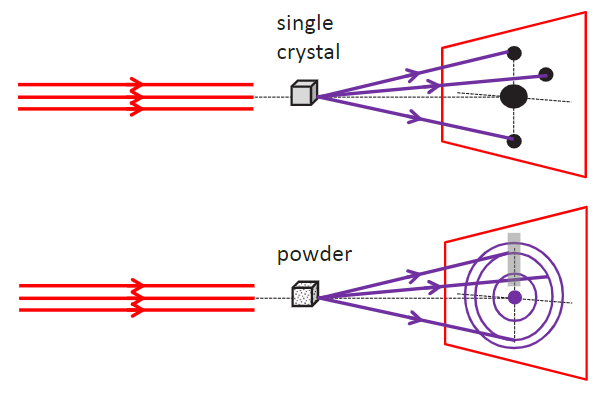
\includegraphics[width=0.309\textwidth]{Lec19/A powder sample contains tens of thousands of randomly oriented crystallites.}
    \caption{A powder sample contains tens of thousands of randomly oriented crystallites.}
\end{figure}
